\documentclass[11pt,onside]{report}
\usepackage{a4}
\usepackage[a4paper,inner=1.5cm,outer=1.5cm,tmargin=3cm, bmargin=3cm,headsep=1.0cm,bindingoffset=0cm,headheight=14pt]{geometry}
\usepackage[onehalfspacing]{setspace}
\usepackage[utf8]{inputenc}
\usepackage[american]{babel}
\usepackage{fancyhdr}
\pagestyle{fancy}
\fancyhead[RO,LE]{\thepage}
\fancyfoot[C]{\vspace{3pt} \thepage}



\usepackage{multirow}
\usepackage[bf,format=plain]{caption}
\usepackage{xcolor}
\usepackage{graphicx}
\usepackage{wallpaper}
\usepackage{wrapfig}
\usepackage{subfig}
\captionsetup[subfloat]{labelfont={footnotesize,rm,md,up}}
\usepackage{float}
\usepackage{booktabs}
\usepackage{enumitem}

\usepackage{latexsym,exscale,amssymb,amsmath,amsfonts,amstext,amsbsy,esint}
\usepackage[thinspace,thickqspace,squaren]{SIunits}

\usepackage[babel]{csquotes}


\usepackage[framed]{matlab-prettifier}


\usepackage[
bookmarks=true,
allcolors=black,
allbordercolors=black,
colorlinks=true,
linkcolor=black,
urlcolor=blue,
pdfauthor={Jan Thiart, Simon Christoph Stein},
pdftitle={TrackNTrace - Manual},
pdfsubject={Manual},
pdfcreator={Jan Thiart},
pdfkeywords={}]
{hyperref}

%%%%%%%%%%%%%%%%%%%%%%%%%% Definitionen %%%%%%%%%%%%%%%%%%%%%%%%%%


\newcommand{\D}[0]{\text{d}}
\newcommand{\N}{\ensuremath{{\vec{\nabla}}}}
\newcommand{\laplace}{\ensuremath{{\underline{\Delta}}}}
\newcommand{\ssection}[1]{\vspace{5mm} \section{#1}}
\newcommand{\ssubsection}[1]{\vspace{5mm} \subsection{#1}}
\newcommand{\scite}[1]{\citep{#1}}
\renewcommand*{\vec}[1]{\ensuremath{\mathrm{\mathbf{{#1}}}}}
\newcommand*{\svec}[1]{\ensuremath{\boldsymbol{{#1}}}}



\numberwithin{equation}{chapter}
% \numberwithin{figure}{chapter}
\renewcommand{\thesection}{\arabic{section}}


% \renewcommand*\thefigure{\thesection.\arabic{figure}}
\renewcommand*\thesubfigure{\alph{subfigure}}
\makeatletter
\renewcommand\p@subfigure{\thefigure}
\makeatother
\setcounter{lofdepth}{2}

\setcounter{secnumdepth}{3}
\setcounter{tocdepth}{3}





\setlength{\parindent}{0pt}

\hyphenation{TrackNTrace}

\newcommand{\executeiffilenewer}[3]{%
\ifnum\pdfstrcmp{\pdffilemoddate{#1}}%
{\pdffilemoddate{#2}}>0%
{\immediate\write18{#3}}\fi%
}
\newcommand{\includesvg}[1]{%
\executeiffilenewer{#1.svg}{#1.pdf}%
{inkscape -z -D --file=#1.svg %
--export-pdf=#1.pdf --export-latex}%
\input{#1.pdf_tex}%
}




\makeatletter
\gdef\tshortstack{\@ifnextchar[\@tshortstack{\@tshortstack[c]}}
\gdef\@tshortstack[#1]{%
  \leavevmode
  \vtop\bgroup
    \baselineskip-\p@\lineskip 3\p@
    \let\mb@l\hss\let\mb@r\hss
    \expandafter\let\csname mb@#1\endcsname\relax
    \let\\\@stackcr
    \@ishortstack}
\makeatother


\def\CC{{C\nolinebreak[4]\hspace{-.05em}\raisebox{.3ex}{\tiny\bf ++}}}





%%%%%%%%%%%%%%%%%%%%%%%%%%%%% Inhalt %%%%%%%%%%%%%%%%%%%%%%%%%%%%%

\begin{document}

\chapter*{TrackNTrace}
\vspace*{-30pt}\textbf{written for MATLAB by Simon Christoph Stein and Jan Thiart}\\ [20pt]
TrackNTrace is a fast, easy-to-use MATLAB framework for single molecule localization, tracking and super-resolution applications. The purpose of this software is to facilitate development, distribution, and comparison of methods in the community by providing an easily extendable, plugin-based system and combining it with an easy-to-use graphical user interface (GUI). This GUI incorporates possibilities for quick inspection of localization and tracking results, giving direct feedback of the quality achieved with the chosen algorithms and parameter values, as well as possible errors, a feature neglected in most software packages available. The plugin system greatly simplifies adapting and tailoring methods towards any research problem's individual requirements. We provide a set of plugins implementing state-of-the-art methods together with the basic program, alongside tools for common post-processing steps such as STORM image generation, or drift correction. TrackNTrace should be useful to anyone who seeks to combine the speed of established software packages such as rapidSTORM or QuickPALM with the simplicity and direct modifiablity of MATLAB, especially when further post-processing is also done in MATLAB.\\
  
In general, TrackNTrace reads a movie file, corrects for camera artifacts if applicable and obtains a rough guess of all possible positions of bright spots in every image. These position candidates then serve as the basis for a fitting routine which refines these candidates, obtaining position, amplitude and local background. Finally, these fit results are then returned to a particle tracking algorithm which tries to link particles close in time and space to form trajectories.\\[10pt]
This manual will first provide all necessary steps for installation (section~\ref{sec:install}) and explain how to use the GUI (section~\ref{sec:overview}). 
%Some in-depth information about the operation of TrackNTrace is provided in section~\ref{sec:in-depth}.
\begin{table}[!h]
\centering
\caption*{\textbf{Requirements}}
\label{tab:requirements}
\begin{tabular}{p{.2\textwidth} p{.55\textwidth}}
\toprule
OS & Windows 7 64-bit or higher, Linux x86\_64 (tested with Kubuntu 14.4) \\[5pt]
MATLAB version & 2013a or higher\\[5pt]
Toolboxes & Image Processing, Statistics, Parallelization (optional) \\[0pt]
\bottomrule
\end{tabular}
\end{table}

Please also note: TrackNTrace currently can only handle single-channel, $\mathrm{2D}+\mathrm{t}$ Tif image stacks. Convert your experimental data accordingly. \clearpage%

\tableofcontents \clearpage

\section{Installation}\label{sec:install}
TrackNTrace is available via a version-controlled git repository at \url{link/to/git/repo}. The first step is not necessary if git is already installed on your system.
\subsection{Windows}
\begin{enumerate}
\item Download and install git which is available at \url{http://git-scm.com}.
\item Open a git bash and clone the repository via \texttt{git clone link/to/repo} .
\item Install the Visual Studio 2012 \CC~Redistributable (x64). This can either be found in the TrackNTrace folder \texttt{external\textbackslash vcredist\textunderscore x64.exe} or downloaded from the Microsoft website \href{https://www.microsoft.com/en-us/download/details.aspx?id=30679}{here}.
\item Open MATLAB, move to the TrackNTrace folder, and execute \texttt{RunTrackNTrace}.
\end{enumerate}

\subsection{Linux (tested with Kubuntu 14.4)}
\begin{enumerate}
\item Install git it via your package manager (e.g. \texttt{sudo apt get install git}).
\item Open a terminal in your home folder and clone the repository via \texttt{git clone link/to/repo} .
\item Open MATLAB, move to the TrackNTrace folder, and execute \texttt{RunTrackNTrace}.
\item Depending on your MATLAB version, TrackNTrace might run without the need for additional configuration.\\
MATLAB in Linux comes with its own \CC~standard library, which might be too old and not compatible with the shared libraries used by ceres. As MATLAB loads its own STL before the system libraries (by setting \texttt{LD\textunderscore LIBRARY\textunderscore PATH} to a MATLAB library directory) this will result  in failures when the mex file (shared library) is called. If you encounter invalid mex files while executing the program or runtime linking errors try setting the \texttt{LD\_PRELOAD} environment variable to the directory with your system libraries (where \texttt{libstdc++} and \texttt{libgfortran} are located; try either the \texttt{locate} command or \texttt{find/ -name} to find them) before starting MATLAB. If you still encounter problems, consider installing the ceres dependencies (see \url{http://ceres-solver.org/building.html}, Linux).
\end{enumerate}
\clearpage

\section{Overview}\label{sec:overview}
Before reading this manual a note: To make TrackNTrace easy to use, we want to emphasize that every UI element has a tooltip explanation, which pops out when resting the mouse on top of the element. Ideally these explanations should be enough to use the program/plugin efficiently.\\

Some of the general behavior of the TrackNTrace software can be altered by individual users by editing the \texttt{getDefaultOptions.m} file. For example, the default plugins on startup can be selected and it can be choosen if the program should use parallel processing or not.

\begin{figure}[!h]
\centering
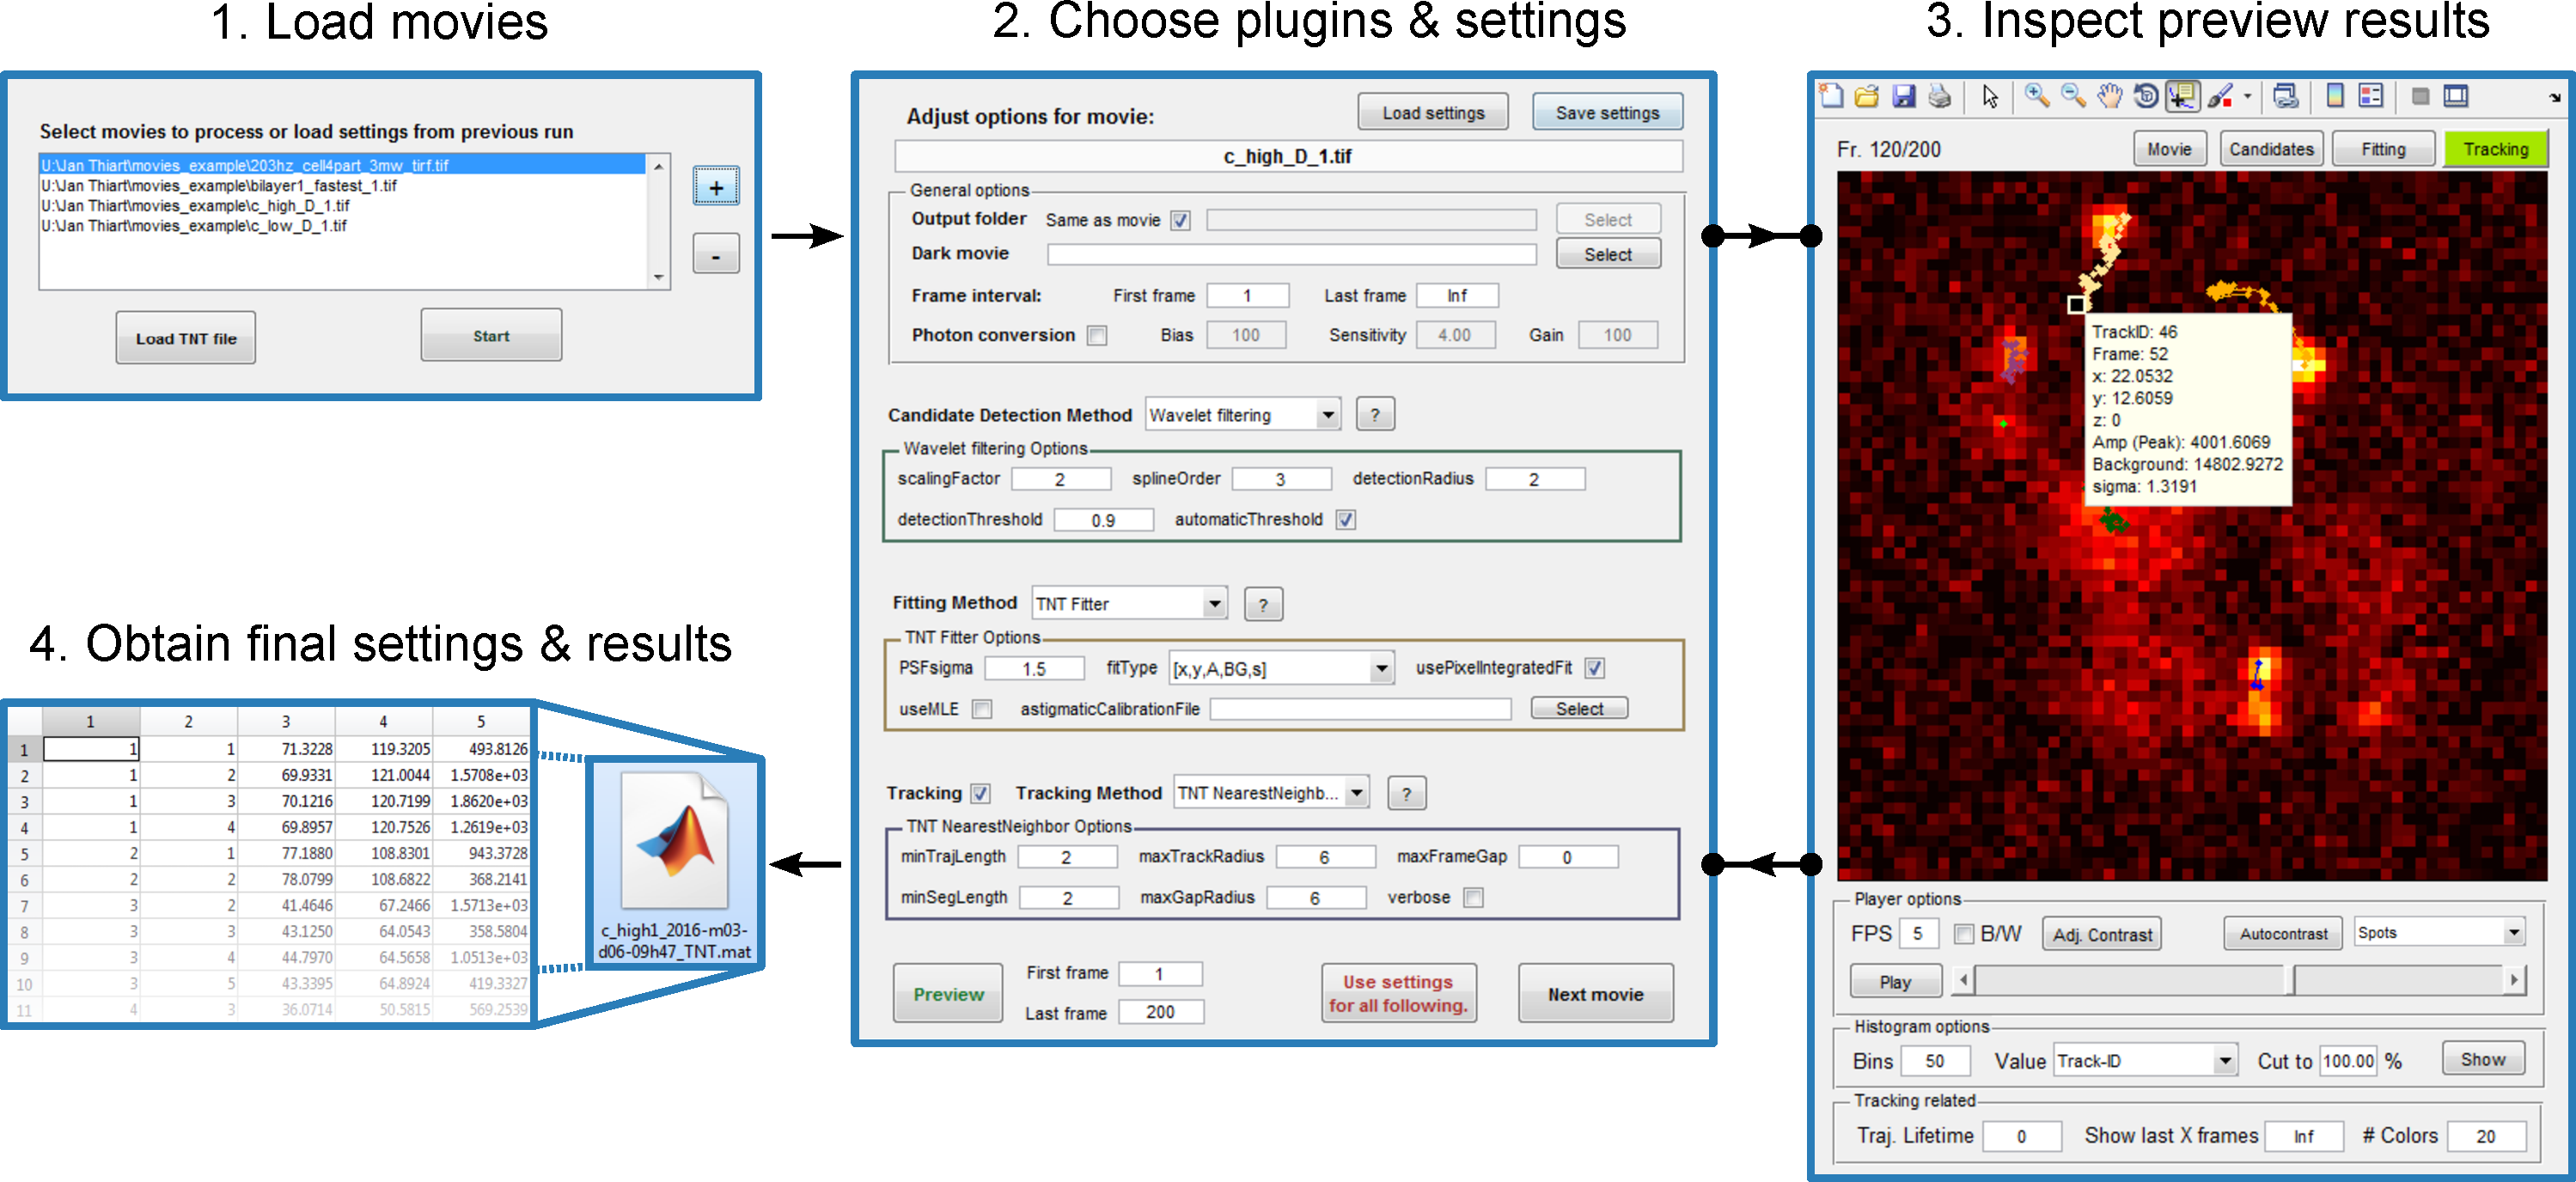
\includegraphics[width=0.9\textwidth]{./fig0.pdf} 
\caption{Program flow and user interface of TrackNTrace. First, a list of movies or a previously saved settings file is loaded before the main GUI is initialized. There, plugins for candidate detection, position refinement, and particle tracking are chosen and their settings adjusted for each movie. At any time during parameter tuning, a preview for an arbitrary part of the current movie can be computed and visualized. The visualizer is able to display the output from all stages (here shown in tracking mode). Selecting a candidate, localization, or track showcases the respective plugin-specific output (e.g. fitted parameter values). After parameter adjustment for all movies, the actual processing starts, saving each movie's output data along with the chosen settings in a single file.}
\label{fig:flowdiagram}
\end{figure}

\subsection{Startup (Fig. \ref{fig:flowdiagram}.1)}
When you first run \texttt{RunTrackNTrace.m}, the GUI as seen in figure~\ref{fig:flowdiagram}.1 pops up. Here, you can select the relevant movie files to process. Movies are added via the ``\textsf{+}'' button, where multiple movies can be selected in one go using the ``\textsf{Shift}'' key. Likewise, the ``\textsf{-}'' button removes the selected entry from the list. Pressing \textsf{Start} invokes the main GUI (fig. \ref{fig:flowdiagram}.2). If ``\textsf{Load TNT file}'' is pressed, a TrackNTrace settings file (MATLAB's \texttt{*.mat} file format, files end on \texttt{\textunderscore TNT}) can be selected, which loads all settings from a previous run, also starting the main GUI.

\subsection{Main GUI (Fig. \ref{fig:flowdiagram}.2)}
In the main GUI all processing settings are adjusted. On first startup it always shows the settings for the first movie in the list. The current settings can be saved to a file or previously saved settings loaded via the \textsf{Save Settings} and \textsf{Load settings} buttons on the top. Below the current file's name is displayed (hovering reveals full path). The main part of the GUI is designed for four processing steps:
\begin{enumerate}
 \item \textbf{Correcting raw data:} Measurements can be corrected for dark currents and camera artifacts. Algorithms based on quantitative analysis of photon signals (e.g. maximum-likelihood estimation, MLE) require subsequent conversion of analogue-digital-converter counts to photon numbers.
 \item \textbf{Detecting candidates:} Potential sources of signal above the background noise are identified in each frame to obtain rough estimates of emitter positions with pixel precision. %This step is critical as misses or false detections cannot be distinguished from true events lateer.
  \item \textbf{Position refinement:} Each candidate's position estimate is refined with sub-pixel accuracy and additional information (background strength, brightness, dipole orientation, etc.) extracted. Commonly, this involves fitting a representation of the microscope's PSF to a subsection of the frame.
    \item \textbf{Tracking:} Positions separated in time are connected frame-by-frame to form trajectories. High particle density, intersecting tracks, and re-appearing, previously lost emitters are the main obstacles to overcome during this stage.
\end{enumerate}

The first part corresponds to the \textsf{General options} panel, where the following elements can be adjusted:
\begin{itemize}[leftmargin=3.5cm]
\item[\textsf{Output folder}] Folder where the TNT output file is saved. The filename is always derived from the movies name with an additional timestamp and the ending \texttt{\textunderscore TNT}. For example: the output of a movie ``\texttt{data.tif}'' could become ``\texttt{data\textunderscore 2016-m03-d14-13h15\textunderscore TNT.mat}''. If \textsf{Same as movie} is checked, the output will be right next to the movie. Otherwise press \textsf{Select} to open a file dialogue where you can select a folder (or simply type one into the field directly). Leaving the field empty saves in the current MATLAB location.
\item[\textsf{Dark movie}] Select a movie taken with the exact same camera settings used in your experiment but with the shutter closed. This movie is used to correct for non-isotropic camera sensitivity, dead pixels and other artifacts according to [1].
\item[\textsf{Frame interval}] Select the first and the last movie frame for processing. Anything not in this interval will be discarded. If \textsf{Last frame} is higher than the movie size or set to \textsf{Inf}, the whole movie is processed, starting at \textsf{First frame}.
\item[\textsf{Photon conversion}] If checked, the movie frames are converted from ADC counts to photons before they are handed to the plugins for processing. The conversion formula is
\begin{align}
I_{\texttt{phot}} = (I_{\texttt{ADC}}-\texttt{Bias})\times\texttt{Sensitivity}/\texttt{Gain}.
\end{align}
A conversion of this type is only meaningful for EMCCD cameras. The values for \texttt{Bias}, \texttt{Sensitivity} and \texttt{Gain} should be available in the camera's performance sheet.
\end{itemize}

The lower part houses the plugins for steps 2-4, where the plugin for each step is selected using a popup menu. The [ \textsf{?} ] button besides these menus shows an explanation of the currently selected plugin. Tracking (step 4) can optionally be disabled/enabled, the other two steps are always carried out. That said, the \texttt{Use candidate data} plugin for step 3 simply copies the data from step 2 and converts it to the right output format. As each plugin's inputs are different, we will not explain the plugins here, but rely on their explanation and their tooltip.\\

At the bottom left part of the GUI the preview button is placed, which starts the visualizer (see below) for the frame interval specified by   \textsf{First frame} and \textsf{Last frame} to the right of the button. This visualization is one of TrackNTrace's core features, making data analysis and parameter optimization much easier. The bottom right button either switches to the settings of the next movie in the list (displays ``\textsf{Next movie}) or starts processing all movies (displays ``\textsf{START processing}''). If all movies are alike, the ``\textsf{Use settings for all following}'' button applies the current movie's settings to all yet unadjusted movies in the list and starts the processing directly.\\[10pt]

\subsection{Preview/Visualizer (Fig. \ref{fig:flowdiagram}.3)}
The visualizer shows the data acquired from steps 2 through 4 (if available). Aside from its use by \texttt{RunTrackNTrace.m}, the visualizer can also be started directly by executing \texttt{TNTvisualizer.m} (check the file for the different input options). This is useful for viewing data from previous runs or even just Tif movies. In the top right the type of data to display can be selected. If a data point is selected with the mouse, all corresponding output parameters from the plugin that computed it are shown. The counter in the top left shows the current/maximum frame. Different modes can show different options at the bottom of the player.

\paragraph{Player options}
\begin{itemize}[leftmargin=3cm]
\item[\textsf{FPS}] The frames per second (speed) the movie is played back with when \textsf{Play} is pressed.
\item[\textsf{B/W}] Black/white colormap for displaying the movie.
\item[\textsf{Adj. contrast}] Shows a popup menu which allows manually changing the contrast.
\item[\textsf{Autocontrast}] The contrast is chosen automatically with a method chosen from the popup menu to the right. Similar to the popular \texttt{ImageJ} software, holding the \texttt{Shift} key during playback continously adjusts the contrast.
\item[] Currently included methods are: \\\hspace*{0.35cm}Spots: Emphasize highest 25\% intensity values.\\\hspace*{0.35cm}Min/Max: Contrast spans all values.\\\hspace*{0.35cm}98\% range: Cuts the lower and upper 1\% of intensities. 
\end{itemize} 

\paragraph{Histogram options (unavailable in \textsf{Movie} mode)}
\begin{itemize}[leftmargin=3cm]
\item[\textsf{Bins}] Number of bins the histogram is computed for.
\item[\textsf{Value}] Parameter to histogram. What is available depends on the plugin that computed the current mode's data.
\item[\textsf{Cut to X \%}] Cuts (100-X)/2 \% of data from the lower and upper tails of the distribution before computing the histogram. 
\item[\textsf{Show}] Computes and displays the histogram.
\end{itemize}

\paragraph{Tracking related (only \textsf{Tracking} mode)}
\begin{itemize}[leftmargin=3.5cm]
\item[\textsf{Traj. Lifetime}] Number of frames a trajectory is visible after its detection.
\item[\textsf{Show last X frames}] Shows only the past X frames of each trajectory.
\item[\textsf{\# Colors}] Number of colors the trajectories are displayed in. 
\end{itemize}

\clearpage
\section{TrackNTrace output}\label{sec:datastructures}
All results obtained by TrackNTrace are saved in a \texttt{mat}-file in the format \texttt{'moviename\textunderscore timestamp\textunderscore TNT.mat'}. Here is a list of all variables it contains:
\begin{table}[!h]
\centering
\caption*{\textbf{TrackNTrace data structures}}
\label{tab:datastruct}
\begin{tabular}{p{.22\textwidth} p{.73\textwidth}}
\toprule
\multicolumn{1}{c}{Variable name} & \multicolumn{1}{c}{Description}\\ \midrule
\texttt{filename\textunderscore movie} & String containing full path of movie file. \\[5pt]
\texttt{dark\textunderscore img} & 2D double array containing correction image to be added to each movie frame. \\[5pt]
\texttt{movieSize} & $1\times3$ matrix saving the size of the movie [rowPixel, colPixel, nrFrames] \\[5pt]
\texttt{firstFrame\textunderscore lastFrame} & $1\times2$ matrix [first frame, last frame] saving the first and last processed frame of the movie. This is important if only parts of a movie were read in and processed. \\[5pt]
\texttt{globalOptions} & Struct of general options variables set by the GUI. \\[5pt]
\texttt{candidateOptions} & Struct of candidate options parameters. Also contains the used plugins name and a parameter description for all output columns in \texttt{outParamDescription}. \\[5pt]
\texttt{fittingOptions} & Struct of fitting options parameters. Also contains the used plugins name and a parameter description for all output columns in \texttt{outParamDescription}. \\[5pt]
\texttt{trackingOptions} & Struct of tracking plugin parameters. Also contains the used plugins name and a parameter description for all output columns in \texttt{outParamDescription}. \\[5pt]
\texttt{candidateData} & $n\times 1$ cell array of candidate positions where $n$ is the number of analyzed frames. Each cell contains a $k\times p$ double array, where $p$ is the number of model parameters and $k$ is the maximum amount of particles in the respective frame. Each row represents a unique candidate fit and the column order is $\mu_x$, $\mu_y$. These columns are mandatory for the fitting to work. Plugins can output extra data.\\
\texttt{fittingData} & $n\times 1$ cell array of fitted positions where $n$ is the number of analyzed frames. Each cell contains a $k\times p$ double array, where $p$ is the number of model parameters and $k$ is the maximum amount of particles in the respective frame. Each row represents a unique fit and the column order according to the model PSF is $\mu_x$, $\mu_y$, $\mu_z$, $A$, $B$ (amplitude, background). These five columns are mandatory for most trackers to work correctly in step 4. Plugins can output extra data.\\
\texttt{trackingData} & 2D double array, list of trajectories with columns  [id,frame,$\mu_x$,$\mu_y$,$mu_z$] + additional columns. Every trajectory is given an id, starting at 1, after which the list is sorted. Frame number starts with 1.\\
\bottomrule
\end{tabular}
\end{table}

\clearpage

\section{How to write a TrackNTrace plugin}\label{sec:howto_plugins}
\subsection{Plugin header}
This section explains how plugins are added to the TrackNTrace framework, with a concise demonstration of all features shown in \texttt{plugins\textbackslash pluginDemo.m}. A plugin is defined as a function in a single file named ``\texttt{plugin\_NAME.m}'' inside the \texttt{plugins} subfolder of the TrackNTrace root directory. 

The function inside the file returns a \texttt{TNTplugin} object. In the simplest case, the file content looks like this:
\begin{lstlisting}[style=Matlab-editor]
function [plugin] = plugin_NAME()
name = 'Some candidate plugin';
type = 2; %1 for candidate, 2 for refinement, 3 for tracking
mainFunc = @arbitraryName_main;
outParamDescription = {'OutputVariableName1'; 'OutputVariableName2'};
plugin = TNTplugin(name, type, mainFunc, outParamDescription);
end

function [output] = arbitraryName_main(img, options, currentFrame) 
% Actual algorithm implemented here
end
\end{lstlisting}

While the four parameters used in the constructor are mandatory for every plugin, there are additional parameters that can be set optionally after the object is constructed. Here is a complete list:

\begin{table}[!h]
\centering
\caption*{\textbf{TNTplugin properties}}
\begin{tabular}{p{.25\textwidth} p{.7\textwidth}}
\toprule
\multicolumn{1}{c}{Property} & \multicolumn{1}{c}{Description}\\ \midrule
  \texttt{name} & Plugin name as displayed by the GUI. \\
  \texttt{type} & Integer, type of plugin. 1: Candidate detection, 2: Spot fitting, 3: Tracking \\
  \texttt{mainFunc} & Handle to main function the plugin implementing the actual algorithm. For type 1 and 2 this is called by TrackNTrace in a loop for each individual frame of the input movie. The interface (output/input) of this function depends on the plugin type and must match the TrackNTrace specification (see below). \\
  \texttt{outParamDescription} &  Cell array of strings with description/name of all output parameters (columns) of the plugin \\
 \texttt{info} & Description of the plugin itself. Should describe the method and the general way how to use it. Supports \texttt{sprintf} modifiers directly (e.g. \texttt{\textbackslash n} for new line). \\
  \texttt{initFunc} &  Initialization function which is called once before the main is first executed. \\
  \texttt{postFunc} & Post-processing function which is called after the main function is last executed. \\
  \texttt{useParallelProcessing}&  Boolean. If false, TrackNTrace does not parallelize this plugins main function on a frame-by-frame basis for type 1/2 plugins. Useful if the main function itself is parallelized (e.g. a compiled multithreaded mex file) or if global information is needed (e.g. access to multiple frames of the movie).\\
  \bottomrule
\end{tabular}\\
\end{table}

Parameters which can be adjusted by the GUI are defined by calling the \texttt{add\textunderscore param(par\textunderscore name, par\textunderscore type, par\textunderscore settings, par\textunderscore tooltip )} function of the newly created plugin instance. Let's look at the ``RadialSymmetry'' fitting plugin as an example:
\begin{lstlisting}[style=Matlab-editor]
function [plugin] = plugin_RadialSymmetry()
name = 'Radial symmetry';
type = 2;
mainFunc =  @refinePositions_radialSymmetry;
outParamDescription = {'x';'y';'z';'Amp (Peak)'; 'Background'; 'width'};

% Create the plugin
plugin = TNTplugin(name, type, mainFunc, outParamDescription);

% Description of plugin
plugin.info = ['Particle localization by radial symmetry centers. \n', ...
               'Algorithm published in Parthasarathy, NatMet 2012(9).'];
% Add parameters
plugin.add_param('PSFSigma',...
    'float',...
    {1.3,0,inf},...
    'PSF standard deviation in [pixel]. FWHM = 2*sqrt(2*log(2))*sigma.');
plugin.add_param('estimateWidth',...
    'bool',...
    true,...
    'Estimate particle width.');
end
\end{lstlisting}
 
As you can see, this plugin has two parameters of different types which will be visible in the GUI. Parameters are accessible for the plugins main function via a struct called \texttt{options}, e.g. \texttt{PSFSigma} can be used inside the function as \texttt{options.PSFSigma}. Eventual whitespaces are replaced with underscores and dots within the parameter name are removed. Different parameters need different \texttt{par\textunderscore settings} as the third input. For example, the \texttt{bool} type parameter takes only the default value, while \texttt{float} type parameters need \texttt{\string{default value, lower bound, upper bound\string}}. The complete list of parameter types and needed settings is: 
\begin{table}[!h]
\centering
\begin{tabular}{p{0.135\textwidth} p{0.59\textwidth} p{0.185\textwidth}}
\toprule 
\multicolumn{1}{c}{\texttt{par\textunderscore type}} & \multicolumn{1}{c}{\texttt{par\textunderscore settings}} & \multicolumn{1}{c}{Example} \\ \midrule
  \texttt{\textquotesingle float\textquotesingle}  &Double variable, \texttt{\string{defaultValue, lowerBound, upperBound\string}} & \verb|{1.3,0,inf}| \\
   \texttt{\textquotesingle int\textquotesingle}    &Integer variable, \texttt{\string{defaultValue, lowerBound, upperBound\string}}& \verb|{4,-10,10}|\\
   \texttt{\textquotesingle bool\textquotesingle}   &Boolean variable, \texttt{defaultValue} & \texttt{true}\\
   \texttt{\textquotesingle string\textquotesingle} & String variable, \texttt{\textquotesingle defaultValue\textquotesingle} & \texttt{\textquotesingle @exp\textquotesingle} \\
   \texttt{\textquotesingle list\textquotesingle}  &  Interactive list box, \texttt{\string{\textquotesingle defaultEntry\textquotesingle, \textquotesingle Entry2\textquotesingle,...\string}}   & \texttt{\string{\textquotesingle x\textquotesingle,\textquotesingle [x,y]\textquotesingle\string}} \\
   \texttt{\textquotesingle filechooser\textquotesingle} & Interactive file chooser dialog \texttt{\string{\textquotesingle defaultDir\textquotesingle,\textquotesingle fileEnding\textquotesingle\string}} & \texttt{\string{\textquotesingle C:/Sci/\textquotesingle,\textquotesingle csv\textquotesingle\string}} \\
   \bottomrule
\end{tabular}
\end{table}

The fourth parameter of the \texttt{add\textunderscore param} function is the tooltip shown when hovering over the parameter with the mouse (note: this supports \texttt{sprintf} modifiers, e.g. \texttt{\textbackslash{}n} for new line). 

\subsection{Plugin body}
A plugin must define a main function in \texttt{plugin.mainFunc}, which is called for every movie frame or all positions in the case of tracking. Unless explicitly forbidden, this process is parallelized using the parallelization toolbox.

The main functions have a different interface for every plugin type shown below:
\begin{lstlisting}[style=Matlab-editor]
% Type 1, candidate detection
function [candidates_frame_i] = mainFuncName(img, candidateOptions, i)
%Find candidates in 'i'-th frame 'img' of the processed frame interval using the options struct 'candidateOptions', and return a 2D position array candidates_frame_i with at least two columns for x and y position, one row per candidate
end
  
% Type 2, fitting/refinement
function [fits_frame_i]= mainFuncName(img, candidates_frame_i, fittingOptions, i)
%Refine candidate positions candidates_frame_i in 'i'-th frame 'img' of the processed frame interval using the options struct fittingOptions, and return a 2D position array fits_frame_i with at least five columns for x,y and z position, an intensity and a background value, one row per fitted candidate
end

% Type 3, tracking
function [trackingData] = mainFuncName(fittingData, trackingOptions);
        %OR
function [trackingData, trackingOptions] = mainFuncName(fittingData,trackingOptions);
%Track the positions in the cell array fittingData (cells of 2D arrays fits_frame) using the options struct trackingOptions and return a 2D array trackingData which should have at least the columns [track_id,frame,x,y,z]. Optionally also return trackingOptions
end
\end{lstlisting}
Note that all variable names are arbitrary, however, their usage/order, their output structure, and their number has to match the above specifications. If your plugin cannot provide some output, e.g. a $z$-position or a background value, use 0 instead. 

If you already have a function \texttt{MyFunction.m} which, for example, finds candidates in an image and expects two parameters \texttt{p1} and \texttt{p2} which have been defined in the plugin header and saved in candidateOptions accordingly, adding the interface is very simple and could look like this:
\begin{lstlisting}[style=Matlab-editor]
function [candidate_xy] = wrapperForMyFunction(img, options, currentFrame)
candidates_xy = MyFunction(img,candidateOptions.p1,candidateOptions.p2);
end
\end{lstlisting}

\subsection{Optional pre- and post-processing functions}
The main functions are executed for every movie frame or all positions in the case of tracking. To avoid having to calculate derived parameters thousands of times althrough they are the same for all frames, or to perform post-processing steps which are only possible once the whole movie is processed, TrackNTrace can execute pre- and post-processing functions defined in \texttt{plugin.initFunc} and \texttt{plugin.postFunc}, if they are available. These functions are called just before or after the main function, respectively:
\begin{lstlisting}[style=Matlab-editor]
function [options] = initFuncName(options)

function [data, options] = postFuncName(data, options)
\end{lstlisting}
The \texttt{initFunc} can alter the \texttt{options} struct or add parameters to it before the main function is executed. This is useful for example for pre-computing masks for filter steps, creating lookup tables, or checking input parameter correctness. The \texttt{postFunc} function can be used to post-process \texttt{data} before it is saved and also add arbitrary information to \texttt{options}. Note that \texttt{data} (either \texttt{candidateData}, \texttt{fittingData}, or \texttt{trackingData}) depends on the plugin type, see Sec.~\ref{sec:datastructures}). 

\subsection{Global variables and parallelization}
If needed, plugin functions can access external data not available to them via a function call by using global variables. Accessible variables are \texttt{globalOptions}, \texttt{candidateOptions}, \texttt{fittingOptions}, \texttt{trackingOptions}, \texttt{movie}, \texttt{filename\textunderscore movie} and \texttt{imgCorrection} as defined in Sec.~\ref{sec:datastructures}. They could be used as such:
\begin{lstlisting}[style=Matlab-editor]
function [output] = fittingFun(img, options, currentFrame)
global globalOptions;
can_use_photons = globalOptions.photonConversion;

if can_use photons
   output = PhotonFun(img,options);
else
   output = NoPhotonFun(img,options);
end

end
\end{lstlisting}
For example, the \texttt{TNT NearestNeighbor} plugin uses global access to \texttt{fittingOptions} to copy the variable \texttt{outParamDescription} of all \texttt{fittingData} columns that are not needed for the tracking. 

Please note: The use of global variables inside type 1/2 plugin functions should be avoided, as functions with global variables can not be frame-by-frame parallelized by TNT, resulting in a possibly much slower execution time. Also note that, for memory reasons, the global \texttt{movie} variable gives access to the 16-bit input movie without photon conversion, regardless of the TrackNTrace settings. If your function both relies on having access to more than the current movie frame and needs a corrected and/or photon-converted movie, use the \texttt{correctMovie} function as in the following example:
\begin{lstlisting}[style=Matlab-editor]
global movie;
arbitaryMovieStack = movie(:,:,1:4);

[correctedStack] = correctMovie(arbitraryMovieStack);
\end{lstlisting}

\clearpage

\section{References}
\begin{itemize}
\item [{[1]}]  Hirsch M, Wareham RJ, Martin-Fernandez ML, Hobson MP, Rolfe DJ: A Stochastic Model for Electron Multiplication Charge-Coupled Devices {--} From Theory to Practice. PLoS ONE 8(1), 2012.
\item [{[2]}] Mortensen, KI, Churchman SL, Spudich, JA, Flyvbjerg H: Optimized localization analysis for single-molecule tracking and super-resolution microscopy. Nature Methods 7, 377 {--} 381, 2010.
\item [{[3]}] Jaqaman K et al: Robust single-particle tracking in live-cell time-lapse sequences. Nature Methods 5, 695 {--} 702, 2008.

\end{itemize}

\end{document}



\section{How TrackNTrace works}\label{sec:in-depth}
After storing all options, reading in the movie and, if applicable, a closed shutter movie for correction, the fitting routine starts. First, the movie frame is cleaned up by adding a correction image obtained from the closed shutter movie as described in [1] and then converted to a photon count image if possible. Then, the respective candidate search function is called for the respective frame and the result is passed to the fit function. Depending on the settings, candidate search is carried out in each frame or only once for the first (or last) frame or an average image of the first few (or last few) frames. In the latter case, fit results from the frame before are passed to the fit function in the next iteration. \\
Two candidate search mechanism are possible: Normalized cross-correlation and intensity filtering. For cross-correlation, a Gaussian PSF mask is created and the \texttt{normxcorr2} function is called to calculate a correlation image of the original movie frame. This image is then processed with a local maximum filter using \texttt{imdilate}. Pixels with a correlation value higher than the user-provided threshold are accepted as spot candidates. In the intensity filtering step, the image is convolved with a normalized filter kernel  consisting of a moving average window and a Gaussian bell curve of $\sigma = \unit{1}{\mathrm{px}}$ against discretization noise before being processed with a local maximum filter. The kernel has a window size of $w = 2r+1$ where $r$ is the spot radius given by the user. Next, a local background image [4] is calculated and all pixels have to pass two tests: The intensity must be among the top $q\%$ in the image and $1-\mathrm{CDF}(\mu_b,\sigma_b) \leq p$ must hold, where CDF ist the normal distribution cumulative density function, and $\mu_b$ and $\sigma_b$ are mean and standard deviation of the local background. $p$ and $q$ are user-provided thresholds.\\[10pt]
A list of spot candidate positions is passed to a \texttt{Mex} file which handles all fitting procedures. First, a square quadrant $I_\mathrm{exp}$ around a candidate pixel is fit to a 2D Gaussian,
\begin{align*}
I_\mathrm{theo}(x,y) = A\exp\left(-\frac{(x-\mu_x)^2}{2\sigma^2} - \frac{(y-\mu_y)^2}{2\sigma^2}\right) + B \quad\mathrm{with}\quad \min_\theta \sum_x\sum_y \left(I_\mathrm{theo}-I_\mathrm{exp}\right)^2
\end{align*}
where $\theta = (A,\mu_x,\mu_y,B,\sigma)$. Fitting $\sigma$ can be disabled by the user. A more accurate model can be obtained by taking into account the finite size of the camera chip pixel grid, where all signal photons hitting any point within a square pixel are accumulated:
\begin{align*}
I_\mathrm{theo, px} &= \int\limits^{+1\slash 2}_{-1\slash 2} \D x \int\limits^{+1\slash 2}_{-1\slash 2} \D y\: I_\mathrm{theo} \\
&= \frac{A \pi \sigma^2}{2}\cdot \left[\mathrm{erfc}\,\left(-\frac{x-\mu_x+1\slash 2}{\sqrt{2} \sigma}\right) - \mathrm{erfc}\,\left(-\frac{x-\mu_x-1\slash 2}{\sqrt{2} \sigma}\right)\right] \times \\
&\quad \left[\mathrm{erfc}\,\left(-\frac{y-\mu_y+1\slash 2}{\sqrt{2} \sigma}\right) - \mathrm{erfc}\,\left(-\frac{y-\mu_y-1\slash 2}{\sqrt{2} \sigma}\right)\right] +B
\end{align*}
Here, $\mathrm{erfc}$ is the complementary error function. Note that $x$- and $y$- dimension are decoupled, meaning that the two terms only have to be calculated once for one column and one line. Residual minimization is done by a Least-squares Levenberg-Marquardt algorithm. The result can be fitted again using Maximum Likelihood Estimation which is proven to yield the best possible result [2]:
\begin{align*}
\min_\theta (-\log\mathcal{L}) = \min_\theta (I_\mathrm{theo}(\theta) - I_\mathrm{exp} \ln I_\mathrm{theo}(\theta))
\end{align*}
All optimization steps rely on the \texttt{ceres-solver} library, an open-source optimization library written in \CC by Google Inc. We chose ceres for its very high performance, great customizability and the possibility of calculating all necessary first-order derivatives by using automatic differentiation which does not require user input and is therefore more robust. The MATLAB implementation by Simon Christoph Stein is available on the MATLAB file exchange where you can also find all necessary files and instructions for building {TrackNTrace}:  \href{http://www.mathworks.com/matlabcentral/fileexchange/52417-fast-gaussian-point-spread-function-fitting--mex-}{http://www.mathworks.com/matlabcentral/fileexchange/52417-fast-gaussian-point-spread-function-fitting--mex-}\\[10pt]
% FIXME \url did not break the url properly, even after trying different options/packages for 20 minutes.. (latex, *rolleyes*)
 After fitting is finished and if tracking is enabled, the result array is converted to a format suitable for the chosen tracker and passed to the tracking routine. Currently there are two options available: u-Track [3], and a custom, highly efficient nearest-neighbor tracker written in \CC. Depending on the tracker, the time complexity of particle linking is at least quadratic in the number of particles, linear in the number of frames and quadratic or even exponential in the number of gap frames. In u-Track's case, splitting the movie into several parts can be much faster than processing all positions in a single batch. In such situations, particles within and directly after such a border or split frame are tracked again to try to re-link trajectory segments artificially cut in half by splitting the movie. Gap frames cannot be accounted for in this case, therefore, caution is advised when using larger gap values and splitting numbers together.\\
For every tracker, the end result is an array containing all trajectories with recorded frame number, and respective $xy$- position and amplitude. Every trajectory has a unique id to facilitate post-processing. \\
While all tracking algorithms are handled more or less the same, u-Track is an exception. u-Track can handle very difficult scenarios such as Brownian-directional motion-switching, particle merging and splitting and provides a large number of user-input variables for this. These options are all hidden in the \texttt{parseUtrackOptions.m} file and are only meant to be changed by an experienced user. Caution is advised.

\clearpage















































